
\subsection{Minimale Netzkonfiguration}
Bei fast allen Betriebssystemen m"ussen w"ahrend der Installation ein paar
Angaben gemacht werden, die "uberall gleichartig sind. In den meisten
Fällen sollte es dabei reichen, wenn man in den Netzwerkeinstellungen
,,IP-Adresse automatisch beziehen'', ,,DHCP verwenden'' oder ähnliches
auswählt. Die Einzelheiten werden für die verschiedenen
Betriebssysteme im Folgenden beschrieben.
\subsubsection{Windows XP}
Man klickt sich durch  über \fbox{Startmenü} $\Rightarrow$
\fbox{Einstellungen} $\Rightarrow$ \fbox{Systemsteuerung} zum Fenster
\fbox{Netzwerkverbindungen} durch:
\centergraphics{bilder/netzwerkverbindungen}
%insert screenshot
Hier ist nun die richtige Netzwerkverbindung auszuwählen. Wie man sie
ermittelt, wird im Abschnitt zur MAC-Adresse beschrieben. Zunächst
sollte man ihren Status überprüfen:  Die Netzwerkverbindung muss
aktiviert sein. Andernfalls muss sie mittels
\fbox{Rechtsklick}$\Rightarrow$\fbox{Aktivieren} aktiviert
werden.  Anschließend ruft man mit
\fbox{Rechtsklick}$\Rightarrow$\fbox{Eigenschaften} das linke Fenster auf:  
\begin{center}
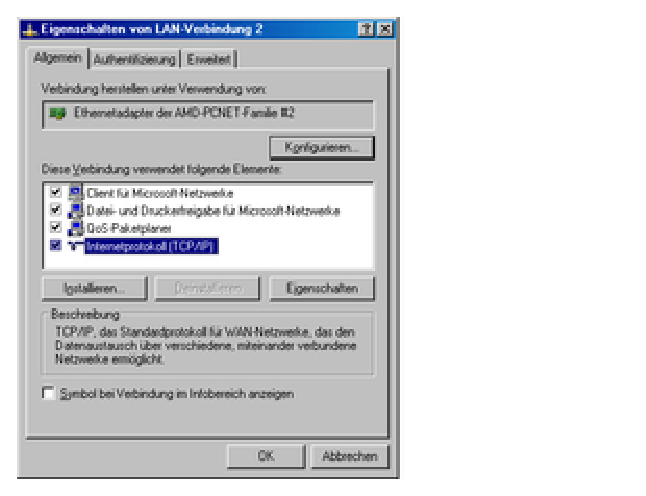
\includegraphics{bilder/eigenschaften_xp}
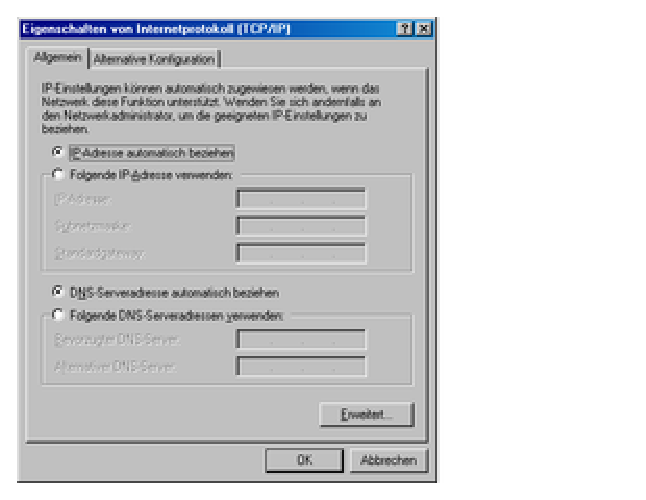
\includegraphics{bilder/dhcp_xp}    
\end{center}
 

Hier ist nun auf \fbox{Internetprotokoll (TCP/IP)} und anschließend
auf \fbox{Eigenschaften} zu klicken. Es sollte sich das rechte Fenster
öffnen.
%und noch einer
Die Einstellungen sollten mit den abgebildeten
übereinstimmen. Andersweitig sind sie zu ändern und mit einen
beherzten Klick auf \fbox{Ok} zu bestätigen. Damit sollte dann in der
Tat alles ok sein.
\subsubsection{Windows Vista/ 7}

\subsubsection{Linux}
\small{Wie schon bei der MAC-Adresse gilt: Je nach Distribution kann es kleinere Unterschiede
geben. Die folgende Anleitung wurde für Debian und Ubuntu getestet und
sollte sich leicht an andere Distributionen anpassen lassen.}
Die folgenden Einstellungen müssen als Administrator (,,root'') vorgenommen
werden. Je nach Distribution ist es dazu erforderlich, sich als root
anzumelden, oder anderweitig als Administrator auszuweisen. In Ubuntu
erfolgt dies beispielsweise mit Hilfe des Programms sudo.\\\\
Die Einstellungen werden durch Bearbeiten der Datei
\texttt{/etc/network/interfaces} vorgenommen. Sie sollte danach
folgende Einträge erhalten:
\begin{verbatim}
# The loopback network interface
auto lo 
iface lo inet loopback
# The primary network interface
auto eth1
iface eth1 inet dhcp 
\end{verbatim}
Dabei muss \texttt{eth1} durch das Kürzel der jeweiligen Netzwerkkarte
ersetzt werden. Wie man diese Netzwerkkarte herausfindet ist im
Abschnitt zur MAC-Adresse beschrieben. Anschließend muss man diese
Änderungen noch aktivieren. Dazu gibt man in eine Konsole nacheinander
folgende Befehle ein:
\begin{verbatim}
ifdown eth1
ifup eth1
\end{verbatim}
Wieder muss \texttt{eth1} durch das entsprechende Kürzel ersetzt
werden. Damit ist die Konfiguration erledigt.

\subsubsection{Testen des Anschlusses}
Sind die Einstellungen erledigt, sollte man die Einstellung
testen. In den meisten Fällen sollte alles klappen. Sollte dies nicht
der Fall sein, gibt es folgende Möglichkeiten: Die mit Abstand
häufigste Fehlerquelle ist es, bei der Anmeldung eine falsche
MAC-Adresse angegeben zu haben. Es empfiehlt sich nun, die
Anmeldebestätigung herauszusuchen und die dort angegebene MAC-Adresse
mit der tatsächlichen zu vergleichen. Sollte man sie vergessen haben
(nicht sooo überraschend bei einer Folge aus hexadezimalen Ziffern),
kann man sie ja mit den aus Abschnitt \ref{sec:netzw-und-mac}
genannten Methoden erneut ermitteln. Sollte sie falsch sein, kann man
die Richtige den Admins in der Sprechstunde oder über eine Email an
\url{admin@schunternet.de} mitteilen\footnote{Wie soll das gehen ohne
  Internet? Hier ist nun Fantasie gefragt: Vom Fragen des Nachbarn,
  über die Computerräume der Uni gibt es ein breites Feld an
  Möglichkeiten :)}.\\\\
Ein anderer häufiger Fehler ist das Benutzen des zweiten
Anschlusses. Jedes Zimmer ist mit einer Dose mit zwei Anschlüssen
ausgestattet. Die Zweite ist im Normalfall aber nicht
freigeschaltet. Dieses Problem sollte sich aber schnell beheben
lassen. Stellenweise sind einige Dosen auch falsch angeschlossen
worden. In so einen Fall sollte man umgehend sich bei uns melden, 
damit entsprechend Abhilfe geschaffen werden kann.\\\\
%Können alle diese Fehler ausgeschlossen werden,  kann man sein Glück
%mit der manuellen Konfiguration der Netzwerkkarte versuchen. 

Können alle diese Fehler ausgeschlossen werden,  sollte man natürlich sich nicht scheuen, uns in der Sprechstunde oder via Mail zu kontaktieren.
%Und
%natürlich ist die Sprechstunde kein Selbstzweck, sondern durchaus
%dafür da, Probleme anzusprechen und dann auch zu lösen :)
%
%%% Local Variables: 
%%% mode: latex
%%% TeX-master: "Netzeinfuehrung"
%%% End: 
